\documentclass[12pt]{article}
\usepackage{stmaryrd}
\usepackage{graphicx} % Pour l'insertion d'images
\usepackage{float}    % Pour contrôler précisément le placement
\usepackage[utf8]{inputenc}

\usepackage[french]{babel}
\usepackage[T1]{fontenc}
\usepackage{hyperref}
\usepackage{verbatim}

\usepackage{color, soul}

\usepackage{pgfplots}
\pgfplotsset{compat=1.15}
\usepackage{mathrsfs}

\usepackage{amsmath}
\usepackage{amsfonts}
\usepackage{amssymb}
\usepackage{tkz-tab}
\author{Destiné aux élèves de Terminale S\\Lycée de Dindéfelo\\Présenté par M. BA}
\title{\textbf{Rappels et compléments sur les fonctions numériques}}
\date{\today}
\usepackage{tikz}
\usetikzlibrary{arrows, shapes.geometric, fit}

% Commande pour la couleur d'accentuation
\newcommand{\myul}[2][black]{\setulcolor{#1}\ul{#2}\setulcolor{black}}
\newcommand\tab[1][1cm]{\hspace*{#1}}

\usepackage[margin=2cm]{geometry}
\usepackage{eso-pic}         % Pour ajouter des éléments en arrière-plan

\usepackage{enumitem}
%---------------------------------------
% Définir un compteur pour les exemples
\newcounter{exemple}

% Définir la commande \exemple pour afficher un exemple numéroté
\newcommand{\exemple}{%
  \refstepcounter{exemple}% Incrémenter le compteur
  \textbf{\textcolor{orange}{Exemple \theexemple : }} \ignorespaces
}
%---------------------------------------
\newcounter{solution}

% Définir la commande \solutione pour afficher un solution numéroté
\newcommand{\solution}{%
  \refstepcounter{solution}% Incrémenter le compteur
  \textbf{\textcolor{orange}{Solution \thesolution : }} \ignorespaces
}
%---------------------------------------
\definecolor{myorange}{rgb}{1.0, 0.8, 0.0}

% Définir un compteur pour les exercices d'application
\newcounter{exerciceapp}

% Définir la commande pour afficher un exercice d'application numéroté
\newcommand{\exerciceapp}{%
  \refstepcounter{exerciceapp}%
  \textbf{\textcolor{myorange}{Exercice d'application \theexerciceapp :}} \ignorespaces
}
%--------------------------------------
% Définir un compteur pour les exercices d'application
\newcounter{correction}

% Définir la commande pour afficher un correction exercice d'application numéroté
\newcommand{\correction}{%
  \refstepcounter{correction}%
  \textbf{\textcolor{myorange}{Correction \thecorrection :}} \ignorespaces
}
%--------------------------------------
% Définir un compteur pour les remarque d'application
\newcounter{remarque}

%----------------------------------------
\definecolor{myorange1}{rgb}{1.0, 1.5, 0}
% Définir la commande pour afficher un remarque numéroté
\newcommand{\remarque}{%
  \refstepcounter{remarque}%
  \textbf{\textcolor{myorange1}{Remarque \theremarque :}} \ignorespaces
}
% Commande pour ajouter du texte en arrière-plan
\AddToShipoutPicture{
    \AtTextCenter{%
        \makebox[0pt]{\rotatebox{45}{\textcolor[gray]{0.9}{\fontsize{5cm}{5cm}\selectfont Pathé Gobel BA}}}
    }
}

\begin{document}
\maketitle
\section*{\underline{\textbf{\textcolor{red}{A. LIMITES-CONTINUITÉ}}}}
\subsection*{\underline{\textbf{\textcolor{red}{I.Limites}}}}

\renewcommand{\labelenumi}{\theenumi)}
\begin{enumerate}[label=\arabic*)]
    \item \textbf{\textcolor{blue}{\underline{Quelques limites usuelles}}}
    
\[\forall n\in\mathbb{N}^{*} \lim_{x \to +\infty} x^{n}=+\infty  \text{ , } \lim_{x \to +\infty} \frac{1}{x^{n}}=0^{+}  \]

\[ \forall n\in\mathbb{N}^{*}
 \lim_{x \to -\infty} x^{n} =
 \begin{cases} 
 +\infty \text{ si \(n\) est pair}\\
 -\infty \text{ si \(n\) est pair}
 \end{cases}
\text{ , }
\lim_{x \to -\infty} \frac{1}{x^{n}}=
 \begin{cases} 
 0^{+} \text{ si \(n\) est pair}\\
 0^{-} \text{ si \(n\) est pair}
 \end{cases}
\]

\[ \lim_{x \to +\infty} \sqrt{x}=+\infty \text{ , } \lim_{x \to +\infty} \frac{1}{\sqrt{x}}=0^{+}  \]

\[ \lim_{x \to a^{+}} \frac{1}{x-a}=+\infty \text{ , } \lim_{x \to a^{-}} \frac{1}{x-a}=-\infty  \]

		\textbf{Autre Notation}
\[( x\rightarrow a^{+} ) \Leftrightarrow ( x\rightarrow a_{>} ) \text{ , } ( x\rightarrow a^{-} ) \Leftrightarrow ( x\rightarrow a_{<} ) \]
\[ \lim_{x \to a^{+}} f(x)=+\infty \text{ se note aussi } \lim_{x \to a_{>}} f(x)=+\infty  \]	

\[ \lim_{x \to a^{-}} f(x)=-\infty \text{ se note aussi } \lim_{x \to a_{<}} f(x)=-\infty  \]	
    
    \item	\textbf{\textcolor{blue}{\underline{Quelques théorèmes sur les limites}}}
\begin{enumerate}[label=\alph*)]
       \item \textcolor{green}{\underline{Théorème de comparaison}}
       
Soient \( f \) et \( g \) trois fonctions définies sur un intervalle \( I \) au voisianage \( \alpha \), \( \alpha \) étant un réel, \( +\infty \) ou \( -\infty \).

\[ \text{Si pour tout \( x\in  I \): }
  \begin{cases}
    f(x)\geq g(x)\\
    \lim_{x \to \alpha}g(x)=+\infty 
  \end{cases}
\text{ alors }  \lim_{x \to \alpha}f(x)=+\infty 
\]

\begin{figure}[H]% Forcer l'image à cet endroit
\centering
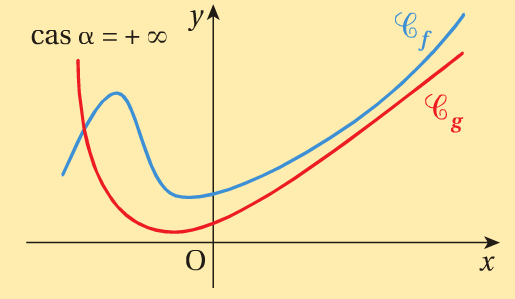
\includegraphics[width=0.8\textwidth]{comp1.png}
\caption{Courbe de (Cf)}
\label{fig:monimage}
\end{figure}

\[ \text{Si pour tout \( x\in  I \): }
  \begin{cases}
    f(x)\leq g(x)\\
    \lim_{x \to \alpha}g(x)=-\infty 
  \end{cases}
\text{ alors }  \lim_{x \to \alpha}f(x)=-\infty 
\]

\begin{figure}[H]% Forcer l'image à cet endroit
\centering
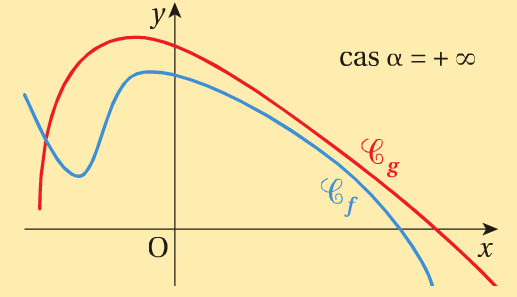
\includegraphics[width=0.8\textwidth]{comp2.png}
\caption{Courbe de (Cf)}
\label{fig:monimage}
\end{figure}

       	\textbf{\underline{\exemple:}}
       	\[ \text{Soit \( f(x)=-x+\sin x \) Calculer }\lim_{x \to +\infty} f(x) \]
       	
       	\newpage
       	\textbf{\underline{\solution:}}
       	\[ \text{Pour tout \(x\), \( \sin x\leq 1 \implies -x + \sin x \leq 1 - x \implies f(x)\leq 1 - x \).} \]
       	\[	\text{Posons \( g(x)=1-x \) donc \( f(x)\leq g(x) \).} \]
       	\[ \text{Or,} \lim_{x \to +\infty}g(x)=-\infty, \text{donc} \lim_{x \to +\infty}f(x)=-\infty\]       	
       	
       	 \textbf{\underline{\exemple:}}
       	\[ \text{Soit \( g(x)=\frac{\sqrt{1+x^{2}}}{x^{2}} \). Calculer }\lim_{x \to 0} g(x) \]
       	 \textbf{\underline{\solution:}}
       	 \[ \text{Posons \( f(x)=\frac{1}{x^{2}} \). Comme, pour tout \(x\neq 0\), on a, \( 1\leq \sqrt{1+x^{2}} \)., on a, pour tout }, x\neq 0 \]
       	\[ f(x)\geq g(x) \text{ Or,} \lim_{x \to 0}g(x)=+\infty, \text{donc} \lim_{x \to 0}f(x)=+\infty\]
       	
       	\item \textcolor{green}{\underline{Théorème d’encadrement ou théorème des gendarmes}}
       	
Soient \( f \), \( g \) et \( h \) trois fonctions définies sur un intervalle \( I \) au voisianage \( \alpha \), \( \alpha \) étant un réel, \( +\infty \) ou \( -\infty \).

\[
\text{ Si \( \forall x\in I \) }
\begin{cases}
  \quad g(x) \leq f(x)\leq h(x) \\
  \lim_{x \to \alpha}g(x)=\lim_{x \to \alpha}h(x)=\ell,
\end{cases}
\text{ alors } \lim_{x \to \alpha}f(x)=\ell 
 \]      	
       	\textbf{\underline{\exerciceapp}}
\[\text{ Calculer } \lim_{ x\to +\infty} \frac{x-\sin x}{x^{2}} \]   	
       	\textbf{\underline{\correction}}
       	
\item \textcolor{green}{\underline{Limite et composition de fonctions}}

Soit \( \alpha \), \( \beta \) et \( \gamma \) des réels ou \( \pm\infty \) On considère deux fonctions \( u \) et \( v \) telles que
	
\[
\text{ Si }
\begin{cases}
  \lim_{x \to \alpha}u(x)=\beta \\
  \lim_{x \to \beta}v(x)=\gamma
\end{cases} 
\text{ alors } \lim_{x \to \alpha}v(u(x))=\gamma 
 \]
       	\textbf{\underline{\exerciceapp}}	
\[\text{Calculer }\lim_{x \to +\infty}\sqrt{\frac{9}{x}+7} \]

				\textbf{\underline{\correction}}
				
On commence par la fonction la plus à l'intérieur :

\[\text{Posons } u(x)=\frac{9}{x}+7 \text{ et } v(x)=\sqrt{\frac{9}{x}+7} \]
				
				
       	\item \textcolor{green}{\underline{Théorème du changement de variable}}
       	\[ \lim_{x \to x_{0}}f(x)=\lim_{t \to 0}f(x_{0}+t) \]
      	\[ \lim_{x \to +\infty}f(x)=\lim_{X \to 0^{+}}f \left( \frac{1}{X} \right)  \]
       	\[ \lim_{x \to -\infty}f(x)=\lim_{X \to 0^{-}}f \left( \frac{1}{X} \right)  \]
       	\textbf{Preuve[Exercice]}    	
			       	
\end{enumerate}
\item \textcolor{green}{\underline{Limites de fonctions trigonométriques}}      
       	\begin{itemize}
       	\item \[ \lim_{x \to 0} \frac{\sin x}{x}=1 \]
       	\item \[ \lim_{x \to 0} \frac{\tan x}{x}=1 \]
       	\item \[ \lim_{x \to 0} \frac{1-\cos x}{x^{2}}=\frac{1}{2} \]
       	\item \[ \lim_{x \to 0} \frac{\cos x -1 }{x}=0 \]
       	\end{itemize}

      	\textbf{\underline{\exerciceapp}}

				 \[ \lim_{x \to +\infty}x\sin \frac{1}{x} \] 
				 \[ \lim_{x \to +\infty}x\tan \frac{3}{x} \] 
				 \[ \lim_{x \to +\infty}x^{2}\left( 1 - \cos \frac{2}{x} \right) \] 	

				\textbf{\underline{\correction}} 

\item \textbf{\textcolor{blue}{\underline{Interprétations géométriques des limites}}}

Les limites peuvent être interprétées géométriquement de plusieurs manières en fonction du contexte. Voici quelques exemples typiques :

\begin{enumerate}[label=\alph*)]
   \item \textcolor{green}{\underline{\textbf{Asymptote horizontale (AH)[Parllèle à \((ox)\)]}}}:
    
\[
\text{ Une fonction }  f  \text{ a une asymptote horizontale en } y = \ell \text{ lorsque} \lim_{x \to +\infty} f(x) = \ell \text{ ou } \lim_{x \to +\infty} f(x) = \ell
\]
\[
\text{ Si } \lim_{x \to +\infty} f(x) = \ell \text{ On dit que: \( y = \ell \) est une AH à \( (C_{f}) \) en }+\infty
\]
    
\[
\text{ Si } \lim_{x \to -\infty} f(x) = \ell\text{ on dit que: \( y = \ell \) est une AH à \( (C_{f}) \) en }-\infty
\]
    
    Cela signifie que la courbe de la fonction se rapproche de la droite \( y = \ell \) à mesure que \( x \to +\infty \) ou \( x \to -\infty \).
    
\textbf{\underline{\exemple:}}

Déterminer l'AH de \( f \)
\[
    f(x) = \frac{2x^2}{x^2 + 1}
\] 
\textbf{\underline{\solution:}}
\[
\lim_{x \to +\infty} f(x) = 2, \quad \lim_{x \to -\infty} f(x) = 2.
\]
    La courbe de la fonction se rapproche de la droite \( y = 2 \) à mesure que \( x \to +\infty \) ou \( x \to -\infty \).
    \item \textcolor{green}{\underline{\textbf{Asymptote verticale (AV)[Parllèle à \((oy)\)]}}} :
    
    Soit \( x = a \in \mathbb{R} \) 
    \[
    \text{si }\lim_{x \to a} f(x) = \pm\infty \text{ alors \(x = a\) est une AV à \(C_{f}\)}
    \]
    Cela signifie que la courbe de la fonction tend vers l'infini lorsque \( x \) approche \( a \) par la droite (ou la gauche).

\textbf{\underline{\exemple:}}

Déterminer de l'AV de \( f \) tel que
\( f(x) = \frac{1}{x} \)

\textbf{\underline{\solution:}}
\[
\lim_{x \to 0^{+}} f(x) = +\infty \quad \text{et} \quad \lim_{x \to 0^{-}} f(x) = -\infty,
\]
ce qui signifie que la fonction a une asymptote verticale en \( x = 0 \).
    \item \textcolor{green}{\underline{\textbf{Asymptote oblique (AO)}}} :
\[ \text{Si } \lim_{x \to +\infty} (f(x)-(ax+b)) = 0 \text{ alors \(y = ax+b\) est une AO à \((C_{f})\) en \( +\infty \)} \]
\[  \]
\[ \text{Si } \lim_{x \to -\infty} (f(x)-(ax+b)) = 0 \text{ alors \(y = ax+b\) est une AO à \((C_{f})\) en \( -\infty \)} \]
\[  \]
Cette méthode est utilisée pour montrer que \(y=ax+b\) est est une AO

\textbf{\underline{\exemple:}}

Soit \( f(x) = \frac{x^2 + 2x + 1}{x} \) une fonction et \( (C_{f}) \) sa courbe représentative.

Montrer que \( y = x + 2 \) est AO à \( (C_{f}) \) en \( \pm\infty \)

\textbf{\underline{\solution:}}

\( y = x + 2 \) est AO à \( (C_{f}) \) en \( \pm\infty \) si
\(\lim_{x \to +\infty}\left[ f(x)-y\right] =0 \)

En effet
    \[
    f(x) = \frac{x^2 + 2x + 1}{x}, \quad \lim_{x \to +\infty} \left( f(x) - (x + 2) \right) = 0.
    \]
    La courbe de la fonction se rapproche de la droite \( y = x + 2 \) pour \( x \to +\infty \).
\item \textcolor{green}{\underline{\textbf{Propriété 1[Autre façon de montrer que \( y = ax + b \) est une AO]}}}

Soit \( f \) une fonction, \( a, b \) un réel et \( (C_{f}) \) sa courbe représentative .
\[
\text{Si }\lim_{x \to +\infty}f(x)=\pm\infty 
\text{ et }
\lim_{x \to +\infty}\frac{f(x)}{x}=a
\text{ et }
\lim_{x \to +\infty}\left( f(x)-ax\right) =b
\]

\[
\text{ alors }
y = ax + b \text{ est une AO à } (C_{f})\quad en\quad +\infty.
\]
\textbf{\underline{NB:}}

Cette propriété reste valable lorsque \( x\rightarrow -\infty\)

On aura \( y = ax + b \) est une AO à \( (C_{f}) \) en \(-\infty\)

\textbf{\underline{\exerciceapp}}

\begin{enumerate}[label=\arabic*)]

\item Soit \( f(x)=\frac{2x}{\sqrt{x+1}} \)
Déterminer \(Df\) et  montrer que \(x=-1\) est une AV à \( (C_{f}) \).

\item Soit \( g(x)=\sqrt{4x^{2}+1}+2x \)

	\begin{enumerate}[label=\alph*)]
		\item Montrer que \(y = 0\) est une AH à \( (C_{g}) \) en \(-\infty\) 
		\item Montrer que \(y = 4x\) est une AO à \( (C_{g}) \) en \(+\infty\) 
	\end{enumerate}

\end{enumerate}
\textbf{\underline{\correction}}

\item \textcolor{green}{\underline{Branche parabolique de direction (oy)}}
\[
 \text{Si } \lim_{x \to +\infty} f(x) = \pm\infty \text{ et } \lim_{x \to +\infty} \frac{f(x)}{x} = \pm\infty 
 \]
 
\[
\text{ alors \((C_{f})\) admet une branche parabolique de direction  \( (oy) \) en \( +\infty \)} 
 \]
		\textbf{\underline{\remarque}}		

Cette propriété reste valable lorsque 	\(x \rightarrow -\infty\)	
		
\item \textcolor{green}{\underline{Branche parabolique de direction (ox)}}
\[
 \text{Si } \lim_{x \to +\infty} f(x) = \pm\infty \text{ et } \lim_{x \to +\infty} \frac{f(x)}{x} = 0 
 \]
 
\[
\text{ alors \((C_{f})\) admet une branche parabolique de direction  \( (ox) \) en \( +\infty \)} 
 \]
		\textbf{\underline{\remarque}}	
				
Cette propriété reste valable lorsque 	\(x \rightarrow -\infty\)	

\item \textcolor{green}{\underline{Branche parabolique de direction \(y = ax\) (a réel)}}
\[
 \text{Si } \lim_{x \to +\infty} f(x) = \pm\infty \text{ et } \lim_{x \to +\infty} \frac{f(x)}{x} = a \text{ et } \lim_{x \to +\infty} (f(x)-ax) = \pm\infty
 \]
 
\[
\text{ alors \((C_{f})\) admet une branche parabolique de direction  \(y=ax\) en \( +\infty \)} 
\]
		\textbf{\underline{\remarque}}	
				
Cette propriété reste valable lorsque 	\(x \rightarrow -\infty\)	
	
\textbf{\underline{\exerciceapp}}

Étudier les branches infinies des courbes représentatives des fonctions suivantes :
\begin{enumerate}[label=\alph*)]
\item \( f(x)=\frac{2x^{3}-1}{x-1} \)

\item \( g(x)=\sqrt{x^{2}+1}-x \)

\item \( h(x)=x\sqrt{\frac{x+1}{x-1}}\)
\end{enumerate}
\textbf{\underline{\correction}}

\end{enumerate}
		
\end{enumerate}

\subsection*{\underline{\textbf{\textcolor{red}{II.Continuité}}}}

\begin{enumerate}[label=\arabic*)]
\item \textbf{\textcolor{blue}{\underline{Définition}}}

Soit f une fonction definie en \( x_{0} \) on dit que f est continue en \( x_{0} \) si
\( \lim_{x \to x_{0}} f(x)=f(x_{0}) \).

\begin{center}
\underline{\textbf{\textcolor{red}{Revoir}}}
\end{center}

\(\left[
\textbf{\textcolor{red}{\underline{Continuité à gauche et continuité à droite}}} 
\right] \)
			
\(\left[ 
\textbf{\textcolor{red}{\underline{Continuité à gauche et continuité à droite}}} 
\right] \)

\(\left[ 
\textbf{\textcolor{red}{\underline{Prolongement par continuité}}}	
\right] \) 

\(\left[ 		
\textbf{\textcolor{red}{\underline{Continuité sur un intervalle}}}
\right] \) 

\(\left[
\textbf{\textcolor{red}{\underline{Continuité de fonctions usuelles}}}
\right] \)

\(\left[
\textbf{\textcolor{red}{\underline{Opérations sur les fonctions continues}}}
\right] \)
\item \textbf{\textcolor{blue}{\underline{Compositions de deux fonctions continues}}}

Si \( f \) est continue en \(x_{0}\) et \( g \) est continue en \( f(x_{0}) \) alors \( gof \) est continue en \(x_{0}\) donc la composition de deux fonctions continues est une fonction continue.

		\textbf{\underline{\exerciceapp}}

		\begin{enumerate}[label=\alph*)]
			\item Soit 	\( f(x)=\sqrt{|2x^{5}|} \)		

		  	Etudier la continuité de 	\( f \) sur \( \mathbb{R} \)
		  
		 	\item Soit \( f(x)=x\sqrt{1-x} \)
		 
		 		Etudier la continuité de f sur son domaine de définition.
		\end{enumerate}	

		\textbf{\underline{\correction}}
		
\textbf{a) Continuité de \( f(x) = \sqrt{|2x^5|} \) sur \( \mathbb{R} \)}

\textbf{Domaine de définition} : \\
La fonction \( f(x) = \sqrt{|2x^5|} \) est définie pour tous les \( x \in \mathbb{R} \), car l’expression \( |2x^5| \) est toujours positive ou nulle, et la racine carrée d’un nombre positif ou nul est bien définie. Donc, \( f(x) \) est définie sur \( \mathbb{R} \).

\textbf{Étude de la continuité} : \\
La fonction \( f(x) \) est composée des fonctions suivantes :
- \( g(x) = 2x^5 \), une fonction polynomiale, qui est continue partout sur \( \mathbb{R} \).
- \( h(x) = |x| \), la fonction valeur absolue, qui est continue partout.
- \( k(x) = \sqrt{x} \), la racine carrée, qui est continue pour \( x \geq 0 \).

Ainsi, \( f(x) \) est continue sur \( \mathbb{R} \), car c’est la composition de fonctions continues sur leur domaine respectif.

\textbf{Conclusion} : La fonction \( f(x) = \sqrt{|2x^5|} \) est continue sur \( \mathbb{R} \).

\textbf{b) Continuité de \( f(x) = x\sqrt{1 - x} \)}

\textbf{Domaine de définition} : \\
La fonction \( f(x) = x\sqrt{1 - x} \) impose que \( 1 - x \geq 0 \), c'est-à-dire \( x \leq 1 \). Ainsi, la fonction est définie pour \( x < 1 \), sans autres contraintes. Le domaine de définition de \( f(x) \) est donc \( ]-\infty, 1[ \).

\textbf{Étude de la continuité} : \\
- La fonction \( g(x) = x \) est continue partout sur \( \mathbb{R} \). \\
- La fonction \( h(x) = \sqrt{1 - x} \) est continue pour \( x < 1 \), car la racine carrée est définie pour les valeurs positives ou nulles. \\
Ainsi, \( f(x) = x\sqrt{1 - x} \) est continue sur \( ]-\infty, 1[ \).

\textbf{Point de discontinuité possible en \( x = 1 \)} : \\
Lorsque \( x \) tend vers 1, la fonction \( \sqrt{1 - x} \) tend vers 0. À \( x = 1 \), la racine carrée devient \( \sqrt{1 - 1} = 0 \), donc \( f(1) = 1 \times 0 = 0 \). Cependant, la fonction n'est pas définie en \( x = 1 \), ce qui entraîne une discontinuité en \( x = 1 \).

\textbf{Conclusion} : La fonction \( f(x) = x\sqrt{1 - x} \) est continue sur \( ]-\infty, 1[ \) et présente une discontinuité en \( x = 1 \).

\item \textbf{\textcolor{blue}{\underline{Image d’un intervalle par une fonction continue et stritement monotone}}}
\begin{itemize}
\item L’image d’un intervalle par une fonction continue est un intervalle.
\[
\text{C’est à dire}
\begin{cases}
\text{\( f \) est continue sur \( I \)}\\
\text{\( I \) est un intervalle}
\end{cases}
\text{alors \( f(I) \) est un intervalle}
\]

\item Lorsqu’une fonction \( f \) est continue et strictement monotone sur \( K \), \( f(K) \) est un intervalle de même nature que \( K \) et ses bornes sont les limites de \( f \) aux bornes de \( K \).

Le tableau ci-dessous précise \( f(K) \) suivant la nature de \( K \) et le sens de variation de \( f \).
\end{itemize}
\begin{tabular}{|c|c|c|c|}
\hline
\( K \) & \( f(K) \) & \( f(K) \)\\
\hline
				& \( f \) stictement croissante & \( f \) strictement décroissante\\
\hline
[a;b]		& \( [f(a);f(b)] \) & \( [f(b);f(a)] \)       \\
\hline
[a;b[	& \( [f(a);\lim_{x\to b^{-}}f(x)[ \) &	\( [\lim_{x\to b^{-}}f(x);f(a)[ \)	\\
\hline
]a;b[		& \( ]\lim_{x\to b^{+}}f(x);\lim_{x\to b^{-}}f(x)[ \) &	\( ]\lim_{x\to b^{-}}f(x);\lim_{x\to b^{+}}f(x)[ \)	\\
\hline
\( [a;+\infty[ \)	& \( [f(a);\lim_{x\to +\infty}f(x)[ \) &\( [\lim_{x\to +\infty}f(x);f(a)[ \)		\\
\hline
\( \mathbb{R} \)& \( ]\lim_{x\to -\infty}f(x);\lim_{x\to +\infty}f(x)[ \)&\( ]\lim_{x\to +\infty}f(x);\lim_{x\to -\infty}f(x)[ \)\\
\hline
\end{tabular}

			\textbf{\underline{\exerciceapp}}
			
				Soit \( f(x)=\frac{2x+1}{x-1} \)
				
				Déterminer l’image par \( f \) des intervalles \( [-2;0] \) et \( ]1;+\infty[ \)
				
			\textbf{\underline{\correction}}
			
\item \textbf{\textcolor{blue}{\underline{Théorème des valeurs intermediaries}}}

Si la fonction \( f \) est \textcolor{red}{ continue }  sur \( [a ; b] \) et si le réel \( m \) est compris entre \( f(a) \) et \( f(b) \), alors l'équation \( f(x) = m \) admet \textcolor{red}{ au moins } une seule solution dans \( [a ; b] \).

Autrement dit, il existe \textcolor{red}{ au moins } un réel \textcolor{red}{ c } entre \textcolor{red}{ \( a \) } et \textcolor{red}{ \( b \) } tel que \textcolor{red}{ \( f(c) = m \) }

\textbf{\textcolor{blue}{\underline{Ilustration graphique}}}

[Image]

\textbf{\underline{\exemple:}}

Soit la fonction \( f(x)=\frac{1}{2}x^{3}+x-5 \) continue sur \( [-2 ; 4] \).

\textbf{\underline{\solution:}}

\(f( [-2 ; 4] ) = [\lim_{x \to -2} f(x) ; \lim_{x \to 4} f(x)] = [-8,6 ; 11,8] \).

D'après le théorème précédent, comme  \(5\in [-8,6 ; 11,8] \) donc l'équation \( f(x) = 5 \) a une solution dans \( [-2 ; 4] \).

\textbf{\textcolor{blue}{\underline{NB}}}

\begin{itemize}
\item Si \(  m = 0 \) il suffit montrer que \( \lim_{x \to a} f(x) \times \lim_{x \to b} f(x) <0 \)
\item Il faut toujours commencer par montrer que \( f \) est continue.
\end{itemize}

\textbf{\underline{\exerciceapp}}

\( f(x) = 2x^{5} + x^{2} + x + 8 \)

Montrer que l’équation \( f(x) = 0 \) admet au moins une solution dans \( [1 ; 2] \).

\textbf{\underline{\correction}}

\item \textbf{\textcolor{blue}{\underline{Théorème d’existence et d’unicité d’une solution}}}

Si la fonction \( f \) est \textcolor{red}{ continue } et \textcolor{red}{ strictement monotone } (croissante ou bien décroissante) sur \( [a ; b] \). Pour tout réel \( m \) compris entre \( f(a) \) et \( f(b) \), alors l'équation \( f(x) = m \) admet une \textcolor{red}{unique continue } dans \(\alpha\in [a ; b] \).

\textbf{\textcolor{blue}{\underline{Ilustration graphique}}}

[Image]

\textbf{\textcolor{blue}{\underline{Cas particulier}}}

Si la fonction \( f \) réalise une bijection(continue et strictement monotone) de \( [a ; b] \) de plus si \( f(a) \times f(b) < 0 \) alors l'équation \( f(x) =0 \) admet une unique solution \( \alpha \) sur l'intervalle 
\( [a ; b] \).
\textbf{\textcolor{blue}{\underline{Ilustration graphique}}}

[Image]

			\textbf{\underline{\exemple:}}
			
			Soit \( f(x)=x^{3} + x + 1 \)

			Montrer que l’équation \( f(x) = 0 \) admet une unique solution sur \( [-0,8 ; -0,6] \).			
			
			\textbf{\underline{\solution:}}

\item \textbf{\textcolor{blue}{\underline{Théorème d’existence d’une bijection et de sa réciproque}}}

Si \( f \) est continue et strictement monotone sur un intervalle \( I \), alors \( f \) est une bijection de \( I \) vers \( J = f(I) \). Dans ce cas, \( f \) admet une fonction réciproque \( f^{-1} \) qui est également continue et strictement monotone sur l'intervalle \( J \), avec les propriétés suivantes :
\begin{itemize}
    \item La fonction réciproque \( f^{-1} \) est telle que \( f(f^{-1}(y)) = y \) pour tout \( y \in J \) et \( f^{-1}(f(x)) = x \) pour tout \( x \in I \).
    \item La monotonie de \( f^{-1} \) est de même sens que celle de \( f \) si \( f \) est strictement croissante et de sens contraire si \( f \) est strictement décroissante.
\end{itemize}

			\textbf{\underline{\exemple:}}

Considérons la fonction \( f : \mathbb{R} \to \mathbb{R} \) définie par :
\[
f(x) = 2x + 3
\]

\begin{enumerate}
    \item La fonction \( f \) est-elle continue sur \(\mathbb{R}\) ?
    \item La fonction \( f \) est-elle strictement monotone sur \(\mathbb{R}\) ?
    \item La fonction \( f \) est-elle une bijection de \(\mathbb{R}\) vers \(\mathbb{R}\) ?
    \item Déterminer l'expression explicite la fonction réciproque \( f^{-1} \) de la fonction \( f \) ?
    \item La fonction réciproque \( f^{-1} \) est-elle continue et strictement monotone ?
\end{enumerate}

\textbf{\underline{\solution:}}
\begin{enumerate}
    \item Oui, la fonction \( f(x) = 2x + 3 \) est continue sur \(\mathbb{R}\) car elle est une fonction affine (polynomiale de degré 1).
    \item Oui, la fonction \( f \) est strictement croissante sur \(\mathbb{R}\), car sa dérivée est \( f'(x) = 2 > 0 \), ce qui signifie que la pente est positive.
    \item Oui, comme \( f \) est continue et strictement croissante, elle est bijective de \(\mathbb{R}\) vers \(\mathbb{R}\).
    \item Pour trouver la fonction réciproque \( f^{-1} \), nous résolvons l'équation \( y = 2x + 3 \) pour \( x \) :
    \[
    y = 2x + 3 \implies x = \frac{y - 3}{2}
    \]
    Donc, la fonction réciproque est \( f^{-1}(y) = \frac{y - 3}{2} \).
    \item Oui, la fonction réciproque \( f^{-1}(y) = \frac{y - 3}{2} \) est également continue et strictement croissante sur \(\mathbb{R}\) car elle est une fonction affine avec une pente positive.
    \item Calculer \( f^{-1}(5) \)
\end{enumerate}
\item \textbf{\textcolor{blue}{\underline{Calcul de \( f^{-1}(y_{0}) \) sans connaître l'expression de \( f^{-1} \) }}}

Pour calculer \( f^{-1}(y_{0}) \), on résout \( f(x)=y_{0} \).

			\textbf{\underline{\exemple:}}
			
			Soit \( f(x) =\sqrt{x^{2}+3x+x-1} \). On admet que f est une bijection de \( [0 ; +\infty[ \) vers \( [-1 ; +\infty[ \)

Calculer \( f^{-1}(2) \) 			
			
			\textbf{\underline{\solution:}}

\item \textbf{\textcolor{blue}{\underline{Encadrement de la racine \( \alpha \) à \( \epsilon \) près}}}

      \textbf{\textcolor{blue}{\underline{Méthode de dichotomie(Approche par exemple)}}}
      
      Si \( f \) fonction \textcolor{red}{strictement contenu} sur un intervalle \( [a;b] \), telle que \( f(a)\geq 0 \) et \( f(b) \leq 0\); alors il existe au moins un réel \( \alpha \) dans  l'intervalle \( [a;b] \) tel que \( f(\alpha) = 0 \).

L'idée est alors de trouver le signe de \( f \) au \textcolor{red}{ milieu } de \( [a;b] \), et de distinguer les deux cas
\begin{itemize}
\item Si \( f\left( \frac{a+b}{2}\right) \leq 0  \), alors \( \alpha \) est dans l'intervalle 
\( \left[\frac{a+b}{2} ; b \right] \)
\item Sinon \( f\left( \frac{a+b}{2}\right) > 0  \), alors \( \alpha \) est dans l'intervalle 
\( \left[a ; \frac{a+b}{2} \right] \)
\end{itemize}
Dans les deux cas, on a trouvé un intervalle de longueur moité dans lequel est située une racine \( \alpha \) de l'équation \( f(x)=0 \).

On recommence alors avec cet intervalle, et ainsi de suite,jusqu'à ce qu'on trouve une approximation qui nous convienne.

\textbf{\underline{\exerciceapp}}
Soit la fonction \(f(x)=x^{3}-7x \)
\begin{enumerate}[label=\alph*)]
\item Montrer que l'équation \( f(x)=0 \) admet une unique solution \( \alpha \) sur l'intervalle \( [2;4] \).
\item Donner un encadrement de \( \alpha \) à 0.1 près
\end{enumerate}

\textbf{\underline{\correction}}

			\textbf{\textcolor{blue}{\underline{Méthode de balayage(Approche par exemple)[Exercice]}}}			

			%\textbf{\underline{Exercice d'application}}
			
			%\textbf{\underline{Solution}}	


\end{enumerate}
\section*{\underline{\textbf{\textcolor{red}{B.Dérivabilité}}}}
\subsection*{\underline{\textbf{\textcolor{red}{I.Dérivation}}}}
\subsection*{\underline{\textbf{\textcolor{red}{1.Notion de nombre dérivé}}}}

Soit \( f \) une fonction définie sur un intervalle \( K \) contenant \( x_{0} \)

\( f \) est dérivable en ou \( f \) admet un nombre dérivé en \( x_{0} \) si et seulment si \[\lim_{x \to x_{0}}\frac{f(x)-f(x_{0})}{x-x_{0}}=\ell \text{ avec } (\ell \in\mathbb{R})\]. \( \ell \) est appelé le nombre dérivé de \( f \) en \( x_{0} \) et noté \( f'(x_{0}) \).

On a alors :\[\lim_{x \to x_{0}}\frac{f(x)-f(x_{0})}{x-x_{0}}=f'(x_{0})\]

			\textbf{\underline{\exemple:}}
			
Soit \( f(x)=\frac{x}{2x+1} \)	Etudier la dérivabilité de \( f \) en \( -1 \).		
			
			\textbf{\underline{\solution:}}

\subsection*{\underline{\textbf{\textcolor{red}{2.Dérivabilté à gauche-Dérivabilté à droite}}}}

Soit f une fonction définie sur un intervalle I contenant $x_{0}$ et $\ell$ un réel.\\
$f$ est dérivable à gauche de $x_{0}$ si\[\lim_{x \to x_{0}^{-}}\frac{f(x)-f(x_{0})}{x-x_{0}}=\ell\]
$f$ est dérivable à droite de $x_{0}$ si\[\lim_{x \to x_{0}^{+}}\frac{f(x)-f(x_{0})}{x-x_{0}}=\ell\]
$f$ est dérivable en $x_{0}$ si\[\lim_{x \to x_{0}^{-}}\frac{f(x)-f(x_{0})}{x-x_{0}}=\lim_{x \to x_{0}^{+}}\frac{f(x)-f(x_{0})}{x-x_{0}}=\ell\]

NB: On note \( f'_{g}(x) \) la dérivé à gauche et \( f'_{d}(x) \) la dérivé à droite

			\textbf{\underline{\exemple:}}

\( f(x) = x|x-1| \) \( f \) est-elle dérivable en \( f \) ?

			\textbf{\underline{\solution:}}

\subsection*{\underline{\textbf{\textcolor{red}{3.Interprétation géométrique du nombre dérivé}}}}
\begin{itemize}
		\item[•] Si \( f \) est dérivable en \( x_{0} \) alors \( f'(x_{0}) \) existe et \( C_{f} \) admet une tangente au point d’abscisse \( x_{0} \) d'équation : \( y=f'(x_{0})(x-x_{0}) + f(x_{0}) \)
\end{itemize}
\subsection*{\underline{\textbf{\textcolor{red}{4.Dérivabilité sur un intervalle }}}}
\( f \) est dérivable sur \( ]a ; b[ \) si et seulement si \( f \) est dérivable en tout point
de \( ]a ; b[ \) .

\textbf{Propriété}:
\begin{itemize}
\item Toute fonction polynôme est dérivable sur \( \mathbb{R} \) .
\item Toute fonction rationnelle est dérivable sur son ensemble de définition .
\item \(|f|\) est dérivable sur \( I \) si et selement si \( f \) est dérivable sur \( I \) et \( f(x)  \neq 0 \forall x \in  I \)
\item \(\sqrt{f}\) est dérivable sur \( I \) si et selement si \( f \) est dérivable sur \( I \) et \( f(x) >0 \forall x \in I \)
\end{itemize}
\subsection*{\underline{\textbf{\textcolor{red}{5.Dérivée d’une fonction composée}}}}

Soit \( f \) une fonction définie sur un intervalle \( I \) et \( g \) une fonction définie sur un intervalle \( K \) contenant \( f(I) \).

\begin{itemize}
\item Si \( f \) est dérivable en un élément \( x_{0} \) de \( I \) et g dérivable en \( f \) alors 

\( g\circ f \) est dérivable en et on a : \( (g\circ f)'(x_{0}) = g' \circ f(x_{0}) \times  f'(x_{0}) \) 

\item Si \( f \) est dérivable sur \( I \) et \( g \) dérivable sur \( K \) alors \( g\circ f \) est

dérivable sur \( I \) et on a : \( (g\circ f)' = g' \circ f \times  f' \)

\end{itemize}

\subsection*{\underline{\textbf{\textcolor{red}{6.Dérivée de la fonction réciproque }}}}

Soit \( f \) une fonction dérivable et bijective de \( I \to J \)  et \( f^{-1} \) la bijection réciproque donc\\ \( f^{-1'}(y)=\frac{1}{f'(x)} \text{avec } f'(x)\neq 0\)

En effet: 
\[
\begin{array}{c c c c}
f : I \to J & & f^{-1} : J \to I \\
f : x \mapsto y = f(x) & & y \mapsto x = f^{-1}(y)
\end{array}
\]

On a 
\( f^{-1}\circ f(x)=x \implies (f^{-1}\circ f(x))'=x' \implies f^{-1'}(f(x))\times f'(x)=1 \implies f^{-1'}(y)\times f'(x)=1\)
\( \implies f^{-1'}(y) = \frac{1}{f'(x)}\)

\textbf{Propriété}:

\( f^{-1'}(y_{0})=\frac{1}{f'(x_{0})}=\frac{1}{f'(f^{-1}(y_{0}))} \text{avec } f'(x)\neq 0\)
Inégalité des accroissements finis (IAF)

\subsection*{\underline{\textbf{\textcolor{red}{7.Inégalité des accroissements finis (IAF) }}}}

%L'inégalité des accroissements finis (IAF) est un résultat clé en analyse mathématique qui permet d'établir une borne sur la variation d'une fonction entre deux points. Elle s'énonce et se démontre comme suit :

%\subsubsection*{\textbf{\textcolor{red}{7.1 Énoncé de l'IAF}}}



Soit \( f \) une fonction dérivable sur un intervalle \( I \). S’ils existent deux nombres réels \( m \) et \( M \) tels que pour tout \( x \) élément de \( I \), 

\( m(b-a) \leq f(b)-f(a) \leq M(b-a)    \)

\textbf{\exemple}

Soit la fonction \( f(x) = 3x^2 - 2x \) définie et dérivable sur l'intervalle \( I = [1, 4] \). Nous cherchons deux nombres réels \( m \) et \( M \) tels que pour tout \( x \in I \), l'inégalité suivante soit vérifiée :
\[
m(b - a) \leq f(b) - f(a) \leq M(b - a).
\]

\textbf{\solution}

\paragraph{1. Calcul de la dérivée de \( f \)} La dérivée de \( f \) est :
\[
f'(x) = 6x - 2.
\]

\paragraph{2. Recherche des valeurs extrémales de \( f'(x) \) sur \([1, 4]\)} Pour trouver les valeurs de \( m \) et \( M \), il faut déterminer les bornes de la dérivée \( f'(x) \) sur l'intervalle \([1, 4]\).

Calculons \( f'(x) \) aux bornes de l'intervalle :
\[
f'(1) = 6 \times 1 - 2 = 4, \quad f'(4) = 6 \times 4 - 2 = 22.
\]

Ainsi, sur \([1, 4]\), on a :
\[
4 \leq f'(x) \leq 22.
\]

\paragraph{3. Détermination des constantes \( m \) et \( M \)} Nous pouvons choisir \( m = 4 \) (la valeur minimale de \( f'(x) \) sur l'intervalle) et \( M = 22 \) (la valeur maximale de \( f'(x) \) sur l'intervalle).

\paragraph{4. Vérification de l'inégalité} Prenons \( a = 1 \) et \( b = 4 \). Calculons \( f(b) - f(a) \) :
\[
f(4) = 3 \times 4^2 - 2 \times 4 = 48 - 8 = 40,
\]
\[
f(1) = 3 \times 1^2 - 2 \times 1 = 3 - 2 = 1.
\]
Donc :
\[
f(4) - f(1) = 40 - 1 = 39.
\]

Calculons maintenant les bornes de l'inégalité avec \( m \) et \( M \) :
\[
m(b - a) = 4 \times (4 - 1) = 12, \quad M(b - a) = 22 \times (4 - 1) = 66.
\]

On a bien :
\[
12 \leq 39 \leq 66.
\]

\paragraph{5. Conclusion} L'inégalité est vérifiée, ce qui montre que pour la fonction \( f(x) = 3x^2 - 2x \) sur l'intervalle \([1, 4]\), les valeurs de \( m = 4 \) et \( M = 22 \) permettent de borner la différence \( f(b) - f(a) \) en fonction de \( b - a \).

%\subsubsection*{\textbf{\textcolor{red}{7.2 Interprétation Géométrique}}}
%L'IAF fournit une interprétation géométrique de la variation d'une fonction. En effet, elle stipule que la pente moyenne entre deux points \((a, f(a))\) et \((b, f(b))\) est égale à la pente de la tangente à la courbe de la fonction en un point intermédiaire \(c\). Cela permet de mesurer la régularité et les variations d'une fonction sur un intervalle donné.

%\subsubsection*{\textbf{\textcolor{red}{7.3 Conséquences et Applications}}}
%L'inégalité des accroissements finis est particulièrement utile dans divers domaines :
%\begin{itemize}
%    \item \textbf{Calcul des bornes} : Elle permet de majorer la variation d'une fonction, ce qui est essentiel pour les études de continuité et de convergence.
%    \item \textbf{Résolution d'inéquations} : L'IAF est souvent utilisée pour démontrer l'unicité des solutions d'équations différentielles.
%    \item \textbf{Approximation locale} : En analyse numérique, l'IAF est une base pour les méthodes de dérivées bornées et pour estimer l'erreur de certaines approximations.
%\end{itemize}

%\subsubsection*{\textbf{\textcolor{red}{7.5 Remarques et Limitations}}}
%Il est important de noter que l'IAF nécessite que la fonction soit continue sur \([a, b]\) et dérivable sur \( ]a, b[ \). Si ces conditions ne sont pas respectées, l'inégalité peut ne pas s'appliquer. De plus, le choix de l'intervalle peut influencer le résultat obtenu, notamment en ce qui concerne la borne maximale sur la dérivée.

\subsection*{\underline{\textbf{\textcolor{red}{C.Primitives}}}}
\subsection*{\underline{\textbf{\textcolor{red}{Définition}}}}
Soit F une fonction dérivable sur un intervalle I et soit f une fonction définie et continue sur I.
 
On dit que F est une primitive de f sur I si pour tout x élément de I

On a : F'(x)=f(x)

F est une primitive de f sur I si f est la dérivée de F sur I.

\textbf{Théorème (admis)}

Toute fonction continue sur un intervalle I admet une primitive sur I.

\textbf{Remarque : }

Si f admet une primitive sur I alors elle en admet une infinité.

\textbf{Théorème }

Deux primitives d'une même fonction sur un même intervalle diffèrent d'une constante.
 
Donc si F et G sont des primitives de f sur I alors il existe une constante réelle k telle que pour tout x élément de I F(x)=G(x)+k
 
Pour la preuve voir la variation des fonctions avec l'utilisation des dérivées.
 
On en déduit que : 
 
Chacune des primitives de f sur I est déterminée par sa valeur en un point de I.

\textbf{Remarque :  }

Toute primitive de f sur I est dérivable sur I.
 
Il serait utile de connaitre les résultats figurant sur le tableau suivant : 

\begin{table}[h!]
    \centering
    \renewcommand{\arraystretch}{1.5}
    \begin{tabular}{|c|c|c|c|}
        \hline
        \textbf{\( I = \) intervalle de} & \textbf{Remarques ou} & \textbf{Fonction \( f \)} & \textbf{Primitive \( F \) où \( k \) est une} \\
        \textbf{définition de \( f \)} & \textbf{restrictions} & & \textbf{constante réelle} \\
        \hline
        \( I \subset \mathbb{R} \) & & \( x \mapsto 0 \) & \( x \mapsto k \) \\
        \hline
        \( I \subset \mathbb{R} \) & \( a \in \mathbb{R} \) & \( x \mapsto a \) & \( x \mapsto ax + k \) \\
        \hline
        \( I \subset \mathbb{R} \) & \( n \) entier naturel & \( x \mapsto x^n \) & \( x \mapsto \frac{x^{n+1}}{n+1} + k \) \\
        \hline
        \( I \subset \mathbb{R}^* \) & \( n \) entier relatif, \( n \neq -1 \) & \( x \mapsto x^n \) & \( x \mapsto \frac{x^{n+1}}{n+1} + k \) \\
        \hline
        \( I \subset \mathbb{R}^+ \) & \( n \) réel \( n \neq -1 \) & \( x \mapsto x^n \) & \( x \mapsto \frac{x^{n+1}}{n+1} + k \) \\
        \hline
        \( I \subset \mathbb{R}^* \) & & \( x \mapsto \frac{1}{x^2} \) & \( x \mapsto -\frac{1}{x} + k \) \\
        \hline
        \( I \subset \mathbb{R}^+ \) & & \( x \mapsto \frac{1}{\sqrt{x}} \) & \( x \mapsto 2\sqrt{x} + k \) \\
        \hline
        \( I \subset \mathbb{R} \) & & \( x \mapsto \sin x \) & \( x \mapsto -\cos x + k \) \\
        \hline
        \( I \subset \mathbb{R} \) & & \( x \mapsto \cos x \) & \( x \mapsto \sin x + k \) \\
        \hline
        \( I \subset \mathbb{R} \) & & \( x \mapsto \sin(ax+b) \) & \( x \mapsto -\frac{1}{a} \cos(ax+b) + k \) \\
        \hline
        \( I \subset \mathbb{R} \) & & \( x \mapsto \cos(ax+b) \) & \( x \mapsto \frac{1}{a} \sin(ax+b) + k \) \\
        \hline
        \( I \subset \mathbb{R} \setminus \left\{ \frac{\pi}{2} + k\pi \right\} \) & & \( x \mapsto \frac{1}{\cos^2 x} \) & \( x \mapsto \tan x + k \) \\
        \hline
        \( I \subset \mathbb{R} \) & & \( x \mapsto 1 + \tan^2 x \) & \( x \mapsto \tan x + k \) \\
        \hline
        \( I \subset \mathbb{R}^+ \) & \( x \) positif & \( x \mapsto \sqrt{x} \) & \( x \mapsto \frac{2}{3} x^{3/2} + k \) \\
        \hline
        \( I \subset \mathbb{R} \) & & \( x \mapsto (ax+b)^n \) & \( x \mapsto \frac{1}{a} \frac{(ax+b)^{n+1}}{n+1} + k \) \\
        \hline
        \( I \subset \mathbb{R} \) & Avec les mêmes & & \\
        & contraintes sur \( n \) et sur \( (ax+b) \) & & \\
        \hline
    \end{tabular}
    \caption{Tableau des primitives}
\end{table}

Lorsque $U$ désigne une fonction dérivable sur $I$, positive et non nulle dans certains cas, on a :

\[
\frac{U'}{U^2} \text{ a pour primitives } -\frac{1}{U} + k
\]

\[
U' \times U^n \text{ a pour primitives } \frac{U^{n+1}}{n+1} + k
\]

\[
U' \times \sqrt{U} \text{ a pour primitives } \frac{2}{3} U \sqrt{U} + k
\]

\[
\frac{U'}{\sqrt{U}} \text{ a pour primitives } 2 \sqrt{U} + k
\]

\[
\frac{U'}{U^n} \text{ peut être ramenée à la forme } U' \times U^{-n}
\]

\section*{\underline{\textbf{\textcolor{red}{D.ÉTUDES DE FONCTIONS}}}}
\subsection*{\underline{\textbf{\textcolor{red}{1) Courbe de la fonction réciproque}}}}

Soit $f$ une bijection de $I$ vers $J$ et $f^{-1}$ sa bijection réciproque.  
La courbe de $f \ (C_f)$ et la courbe de $f^{-1} \ (C_{f^{-1}})$ sont symétriques par rapport à la première bissectrice  
\[
(\Delta) \text{ d'équation } y = x.
\]
\subsection*{\underline{\textbf{\textcolor{red}{2) Fonction paire}}}}

Soit $f$ une fonction et $D_f$ son ensemble de définition. $f$ est dite paire lorsque pour tout $x$ élément de $D_f$  
\[
\text{On a } -x \in D_f \text{ et } f(-x) = f(x).
\]

\subsection*{\underline{\textbf{\textcolor{red}{2) Fonction impaire}}}}
Soit $f$ une fonction et $D_f$ son ensemble de définition. $f$ est dite impaire lorsque pour tout $x$ élément de $D_f$  
\[
\text{On a } -x \in D_f \text{ et } f(-x) = -f(x).
\]

\subsection*{\underline{\textbf{\textcolor{red}{4) Centre de symétrie}}}}
Le plan est muni d'un repère $(O, I, J)$. $(C_f)$ est la représentation graphique d'une fonction $f$.  

Pour démontrer que le point $A(a ; b)$ est un centre de symétrie de $(C_f)$ on peut procéder comme suit :

\subsubsection*{1ère méthode}
\begin{itemize}
    \item On détermine la fonction $g$ dont la représentation graphique est l'image de $(C_f)$ par la translation de vecteur $\vec{AO}$, cette fonction $g$ est définie par : $g(x) = f(x + a) - b$.
    \item On démontre que $g$ est impaire.
\end{itemize}

\subsubsection*{2ème méthode}
Le point $A(a ; b)$ est un centre de symétrie de $(C_f)$ si et seulement si pour tout $x$ élément de $D_f$  
\[
\text{On a } 2a - x \in D_f \text{ et } f(2a - x) + f(x) = 2b.
\]

\textbf{\underline{\exerciceapp}}
\textbf{\underline{\correction}}
\subsection*{\underline{\textbf{\textcolor{red}{5) Axe de symétrie}}}}

Le plan est muni d’un repère orthogonal $(O, I, J)$. $(C_f)$ est la représentation graphique d’une fonction $f$.

Pour démontrer que la droite $(\Delta)$ d' équation $x = a$ est un axe de symétrie de $(C_f)$ on peut procéder comme suit :

\subsection*{1\textsuperscript{ère} méthode}

\begin{itemize}
    \item On détermine la fonction $g$ dont la représentation graphique est l’image de $(C_f)$ par la translation de vecteur $\overrightarrow{A0}$, $A$ étant le point de coordonnées $A(a; 0)$, cette fonction $g$ est définie par :
    \[
    g(x) = f(x + a)
    \]
    \item On démontre que $g$ est paire.
\end{itemize}

\subsection*{2\textsuperscript{ème} méthode}

La droite $(\Delta)$ d' équation $x = a$ est un axe de symétrie de $(C_f)$ si et seulement pour tout $x$ élément de $D_f$ :
\[
f(2a - x) = f(x).
\]


\subsection*{\underline{\textbf{\textcolor{red}{8) Périodicité}}}}

Soit $f$ une fonction et $D_f$ son ensemble de définition. Soit $T$ un nombre réel strictement positif. On dit que 

$T$ est une période de $f$ lorsque pour tout $x$ élément de $D_f$, on a :

\begin{itemize}
    \item $x + T \in D_f$ \hfill (1)
    \item $f(x + T) = f(x)$ \hfill (2)
\end{itemize}

Le plus petit réel $T$ strictement positif qui vérifie (1) et (2) est appelé la période de $f$.
\subsection*{\underline{\textbf{\textcolor{red}{9) Position relative d’une courbe et de son asymptote \( (\Delta): y = ax + b \)}}}}

Soient $f$ une fonction et $(C_f)$ sa courbe représentative. $(\Delta) : y = ax + b$.

Posons $g(x) = f(x) - (ax + b)$.

\begin{itemize}
    \item Si $g(x) > 0 \ \forall x \in K$, alors $(C_f)$ est au-dessus de $(\Delta)$ sur $K$.
    \item Si $g(x) < 0 \ \forall x \in K$, alors $(C_f)$ est au-dessous (ou en dessous) de $(\Delta)$ sur $K$.
    \item Si $g(x) = 0 \ \forall x \in K$, alors $(C_f)$ et $(\Delta)$ se coupent sur $K$.
\end{itemize}
\subsection*{\underline{\textbf{\textcolor{red}{10) Position relative d’une courbe et de sa tangente au point \( M_{0} \)  d'abscisse \( x_{0} \)}}}}

Soit $f$ une fonction deux fois dérivable sur un intervalle $K$ et $x_0$ un élément de $K$. 

On désigne par $(C_f)$ sa courbe représentative et par $(T)$ la tangente à $(C_f)$ au point $M_0$ d’abscisse $x_0$.

$(T)$ a pour équation : $y = f(x_0) + f'(x_0)(x - x_0)$.

\begin{itemize}
    \item Si $f'' > 0 \ \forall x \in K$, alors $(C_f)$ est au-dessus de $(T)$ sur $K$. On dit que $f$ est convexe sur $K$.
    \item Si $f'' < 0 \ \forall x \in K$, alors $(C_f)$ est au-dessous (ou en dessous) de $(T)$ sur $K$. On dit que $f$ est concave sur $K$.
    \item Si $f''$ s'annule et change de signe en $x_0$, alors la droite $(T)$ traverse la courbe $(C_f)$ en $M_0$. On dit que $M_0$ est un point d’inflexion de $(C_f)$.
\end{itemize}
\section*{PROBLÈME}

Soit $f$ la fonction définie par :
\[
f(x) =
\begin{cases} 
2x\sqrt{1 - x^2} & \text{si } x > 0 \\ 
-x + \sqrt{x^2 - 2x} & \text{si } x \leq 0 
\end{cases}
\]

\begin{enumerate}
    \item Déterminer $D_f$, les limites aux bornes et préciser les asymptotes et branches infinies éventuelles.
    \item Étudier la dérivabilité de $f$ en 0 et 1; interpréter géométriquement les résultats obtenus.
    \item Calculer $f'(x)$ là où $f$ est définie, puis dresser le tableau de variation de $f$.
    \item Tracer la courbe de $f$.
    \item Soit $h$ la restriction de $f$ à l’intervalle $]-\infty ; 0]$.
    \begin{enumerate}
        \item Montrer que $h$ admet une bijection réciproque $h^{-1}$ dont on précisera l’ensemble de définition, l’ensemble de dérivabilité et le tableau de variation.
        \item Sans utiliser l’expression de $h^{-1}(x)$, calculer $(h^{-1})'(2)$.
        \item Déterminer explicitement $h^{-1}$.
        \item Tracer la courbe de $h^{-1}$ dans le même repère que celle de $f$.
    \end{enumerate}
\end{enumerate}

\end{document}
